\documentclass{beamer}
%%% ========== Package setup ==========
\usepackage{xeCJK}      % Chinese words package
\usepackage{fontspec}   % Word fonts package
\usepackage{listings}   % Wrap Figure or table package
\usepackage{wrapfig}    % Multicolumn package
\usepackage{multicol}   % Multicolumn package
\usepackage{pdflscape}  % Landscpae package

%%% ========== Slide setting ==========
%% Slide theme setup
\usetheme{CambridgeUS}
\usecolortheme{wolverine}

%% Setup chinese words encoder
\XeTeXlinebreaklocale "zh"
\XeTeXlinebreakskip = 0pt plus 1pt

%% More word fonts
\setmainfont{Times New Roman}
\renewcommand{\familydefault}{\rmdefault}
\setCJKmainfont{標楷體}

% Setting for figure and table numbering
\setbeamertemplate{caption}[numbered]

%%% ========== Title setup ==========
\date{March 14, 2022}
\title{Meeting}
\author{Po Hsun Wu}

%%% ========== Document ==========
\begin{document}
    \maketitle

    \section{Progress report}

    \begin{frame}
        \frametitle{\secname}

        \begin{itemize}
            \item Install tensorflow package for python.
            \item Try two cases for using Keras API.
        \end{itemize}

    \end{frame}

    \section{Result}

    \begin{frame}
        \frametitle{\secname}

        Target function:
        $$f(x)=x^2$$

        \begin{multicols}{2}
            First case:
            \begin{itemize}
                \item Two hidden layers
                \item Each for 20 neuros
                \item Sigmoid function
            \end{itemize}

            Second case:
            \begin{itemize}
                \item Two hidden layers
                \item Each for 64 neuros
                \item Sigmoid function
            \end{itemize}
            \columnbreak

            Database:
            \begin{itemize}
                \item Input range: $[0,10)$
                \item 1,000,000 random datas
                \item Split into 1000 groups
                \item Train 50 times
            \end{itemize}
        \end{multicols}
    \end{frame}

    \begin{frame}
        \frametitle{\secname}

        \begin{figure}
        \begin{multicols}{2}
                \includegraphics[width=2.2in]{Figs/value.png}
                \caption{f(x) vs x}
                \columnbreak

                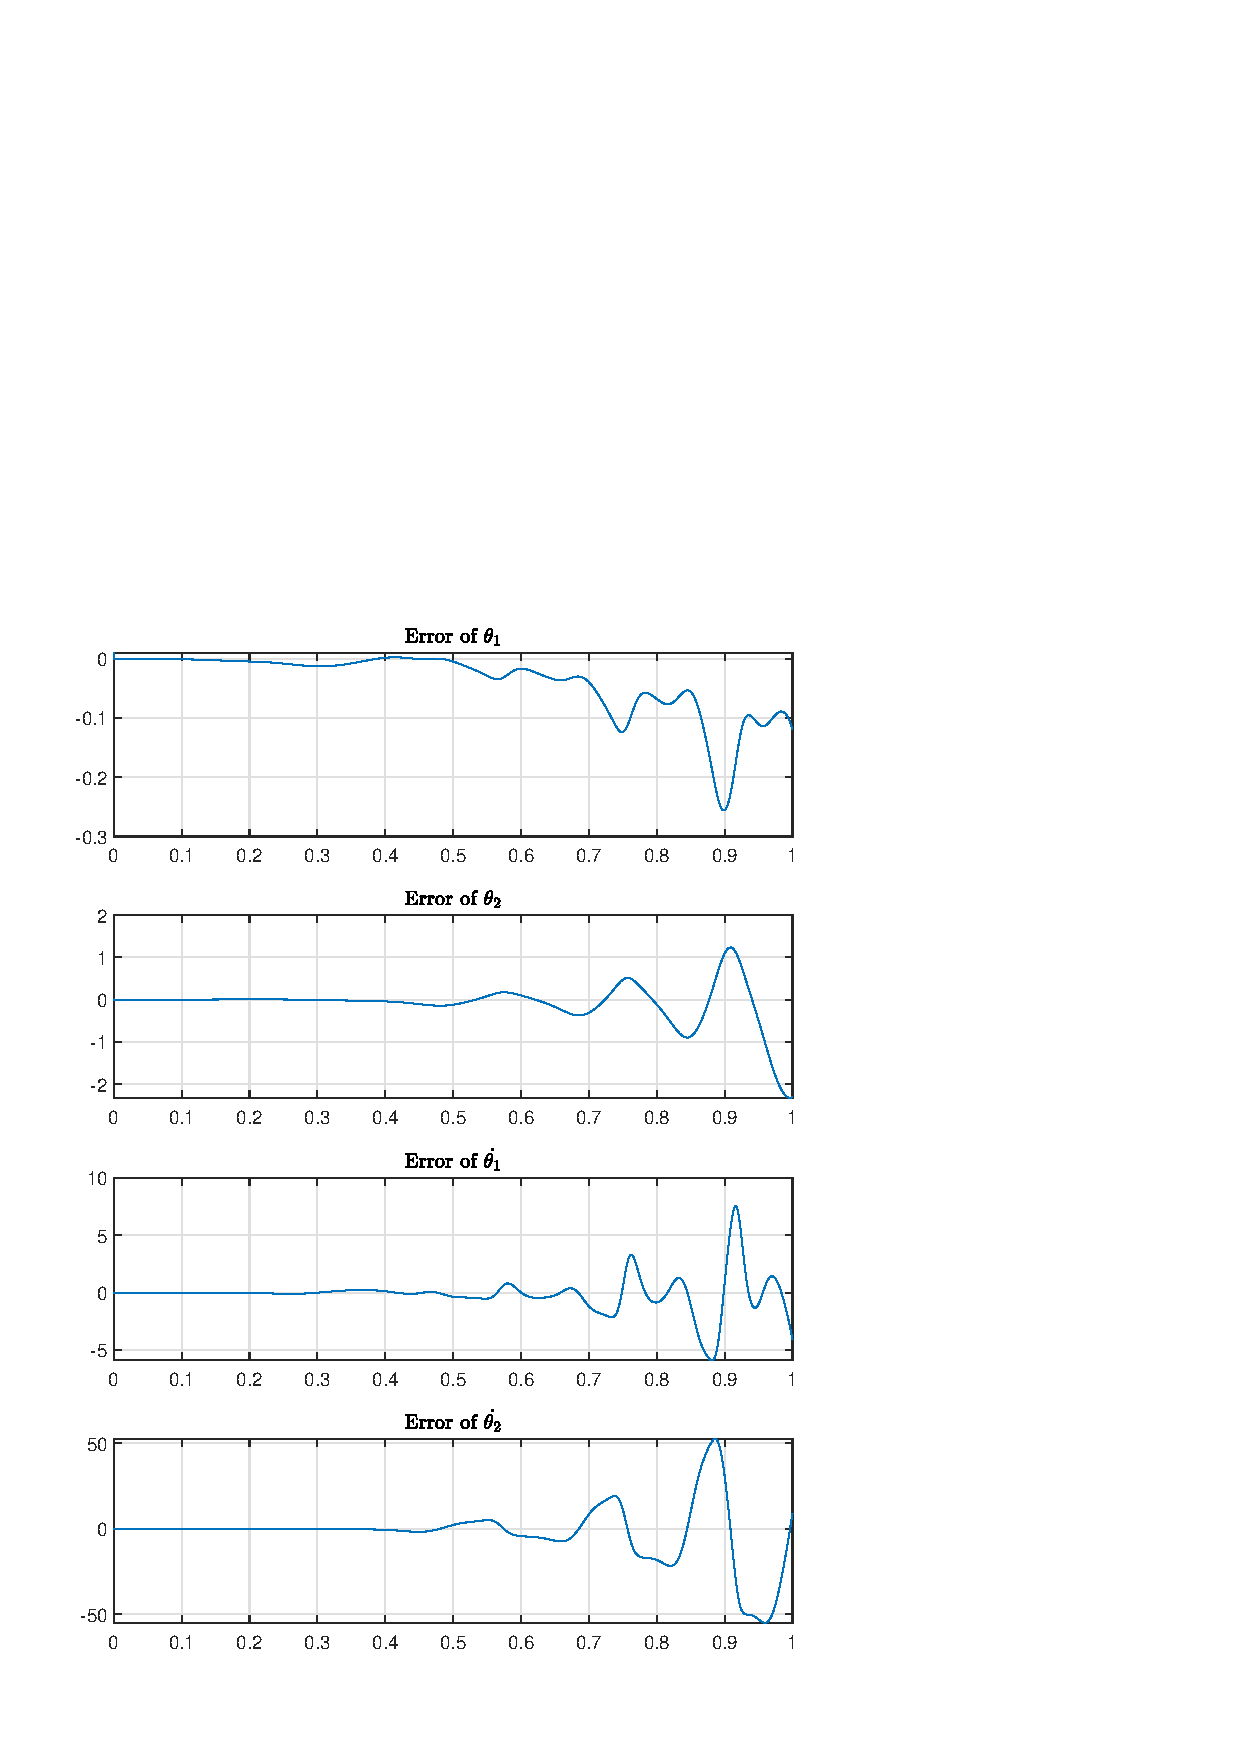
\includegraphics[width=2.2in]{Figs/error.png}
                \caption{Relative error}

            \end{multicols}
        \end{figure}
    \end{frame}

    \section{Source code}

    \begin{landscape}
        \begin{frame}[fragile]
        %   \frametitle{\secname}

            \lstset{
                basicstyle=\fontsize{6.5}{6.5}\selectfont\setmainfont{Consolas},
                keywordstyle=\color{blue},
                numbers=left,
                numbersep=5pt
            }

            \begin{lstlisting}[language=Python]
    from tensorflow.keras.layers import Dense
    from tensorflow.keras.models import Sequential
    import numpy as np

    target_fun = lambda x: x*x

    model = Sequential([
        Dense(units=20, activation="sigmoid", input_dim = 1),
        Dense(units=20, activation="sigmoid"),
        Dense(units=1)
    ])

    model.compile(optimizer='sgd', loss='mse')

    for i in range(2):
        x = np.random.rand(1000000, 1)*10
        y = target_fun(x)

        model.fit(x, y, batch_size=1000, epochs=50)

    y_hat = model.predict(x)
    error = np.average(np.abs(y-y_hat))

    print(np.abs(y-y_hat))
    print(error)
    print(model.predict(np.ones((1,1))))

    model.save("sigmoid_20_twice")
            \end{lstlisting}

        \end{frame}
    \end{landscape}

\end{document}